\documentclass[aspectratio=169]{beamer}

\usetheme[progressbar=frametitle, block=fill]{metropolis}
\usepackage{fontawesome5}
\usepackage{tikz}
\usetikzlibrary{arrows.meta, positioning}
\usepackage{xcolor}

% ── Palette (Clean Modern Tech) ──────────────────────────────────────────────
\definecolor{slate}{RGB}{35, 55, 59}
\definecolor{accent}{RGB}{235, 129, 27}
\definecolor{leanteal}{RGB}{0, 121, 107}
\definecolor{passgreen}{RGB}{34, 139, 34}
\definecolor{failred}{RGB}{180, 0, 0}

\setbeamercolor{block title}{bg=leanteal, fg=white}
\setbeamercolor{block body}{bg=leanteal!8, fg=black}
\setbeamercolor{block title example}{bg=passgreen, fg=white}
\setbeamercolor{block body example}{bg=passgreen!8, fg=black}
\setbeamercolor{block title alerted}{bg=failred, fg=white}
\setbeamercolor{block body alerted}{bg=failred!8, fg=black}

% ── Helper macros ────────────────────────────────────────────────────────────
\newcommand{\statcard}[4]{%
  \begin{tikzpicture}
    \node[draw=#2, fill=#2!8, rounded corners=4pt, line width=0.8pt,
          minimum width=#1, minimum height=2.1cm, align=center]
      {{\huge\bfseries\color{#2} #3}\\[3pt]{\small #4}};
  \end{tikzpicture}}

\newcommand{\chip}[1]{%
  \tikz[baseline=(c.base)]\node[draw=passgreen, fill=passgreen!10,
        rounded corners=3pt, minimum width=6.3cm, minimum height=0.6cm,
        font=\small, anchor=west] (c) {\textcolor{passgreen}{\faCheckCircle}\ #1};}

\title{Question Paper Prediction Engine}
\subtitle{Combinatorial Assembly \& Formally Verified Decision Engine in Lean 4}
\author{Team}
\date{\today}

\begin{document}

% ── 1. Title ─────────────────────────────────────────────────────────────────
\maketitle

% ── 2. What is it? ───────────────────────────────────────────────────────────
\begin{frame}{What is it?}
  \Large\textbf{Combinatorial candidate assembler with formal rule verification.}
  \normalsize\vspace{1.2em}
  \begin{itemize}
    \item[\textcolor{accent}{\faDatabase}] \textbf{Upstream Pre-tagged Pool:} Questions arrive already cleaned, tagged to syllabus, and normalized.
    \item[\textcolor{accent}{\faCogs}] \textbf{Combinatorial Assembly:} Engine builds valid candidate papers across Part A and Part B slots.
    \item[\textcolor{accent}{\faShieldAlt}] \textbf{Proof Gate in Lean 4:} Checks hard constraints; invalid papers are unconditionally rejected.
    \item[\textcolor{accent}{\faStar}] \textbf{Soft Constraint Ranking:} High-scoring verified papers are delivered via API to the Frontend.
  \end{itemize}
\end{frame}

% ── 3. Workflow ──────────────────────────────────────────────────────────────
\begin{frame}{Engine Workflow}
  \centering
  \vspace{0.4em}
  \resizebox{\textwidth}{!}{%
  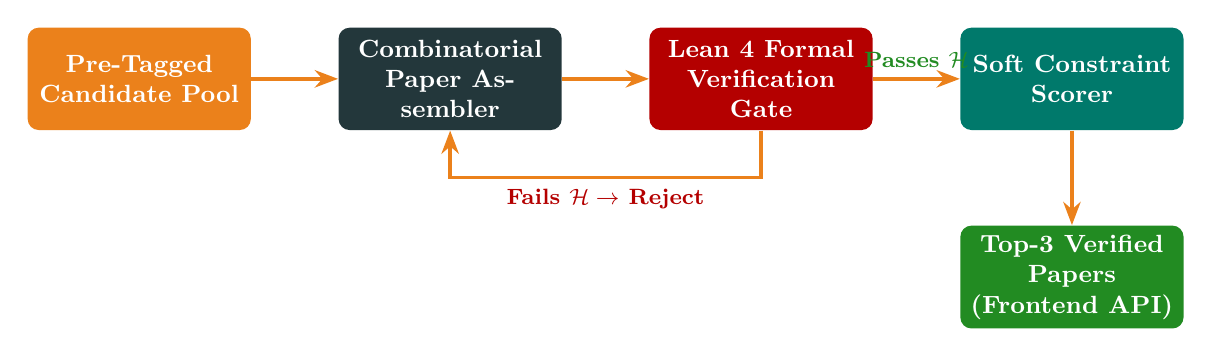
\begin{tikzpicture}[
    node distance=1.1cm,
    stage/.style={rounded corners=4pt, fill=slate, text=white, text width=2.6cm,
                  align=center, minimum height=1.3cm, font=\small\bfseries},
    arrow/.style={-{Stealth}, very thick, color=accent}
  ]
    \node[stage, fill=accent] (A) {Pre-Tagged\\Candidate Pool};
    \node[stage, right=of A] (B) {Combinatorial\\Paper Assembler};
    \node[stage, right=of B, fill=failred] (C) {Lean 4 Formal\\Verification Gate};
    \node[stage, right=of C, fill=leanteal] (D) {Soft Constraint\\Scorer};
    \node[stage, below=1.2cm of D, fill=passgreen] (E) {Top-3 Verified Papers\\(Frontend API)};

    \draw[arrow] (A) -- (B);
    \draw[arrow] (B) -- (C);
    \draw[arrow] (C) -- node[above, font=\footnotesize\bfseries, color=passgreen] {Passes $\mathcal{H}$} (D);
    \draw[arrow] (C.south) -- ++(0,-0.6) -| node[near start, below, font=\footnotesize\bfseries, color=failred] {Fails $\mathcal{H} \to$ Reject} (B.south);
    \draw[arrow] (D) -- (E);
  \end{tikzpicture}}
\end{frame}

% ── 4. How the Engine Works ──────────────────────────────────────────────────
\begin{frame}{How the Engine Works}
  \begin{columns}[T]
    \column{0.48\textwidth}
    \begin{block}{\faThLarge\ 1. Combinatorial Assembly}
      Takes questions from the tagged pool and systematically fills:
      \begin{itemize}
        \item Part A: 10 slots (2 per unit)
        \item Part B: 5 unit pairs (Choice I \& II)
      \end{itemize}
    \end{block}
    \begin{block}{\faShieldAlt\ 2. Lean 4 Verification Gate}
      Evaluates mathematical predicates. \\
      \textbf{If any hard rule is violated $\to$ paper is dropped.}
    \end{block}

    \column{0.48\textwidth}
    \begin{block}{\faBalanceScale\ 3. Soft Constraint Scoring}
      Surviving papers are ranked by:
      \begin{itemize}
        \item Topic frequency \& recency gaps
        \item Bloom's cognitive taxonomy weights
      \end{itemize}
    \end{block}
    \begin{block}{\faDesktop\ 4. API Output to Frontend}
      Emits Top-3 highest-scoring verified blueprints as clean JSON for the UI to display.
    \end{block}
  \end{columns}
\end{frame}

% ── 5. Hard Constraints (The Proving Gate) ────────────────────────────────────
\begin{frame}{The Hard Constraints Proving Gate}
  \begin{block}{Lean 4 Proof Invariants ($\mathcal{H}$)}
    A paper is assembled from the candidate pool; Lean evaluates Boolean invariants. \\
    \textbf{If any constraint fails $\to$ paper is rejected immediately.}
  \end{block}
  \vspace{0.4em}
  \begin{columns}[T]
    \column{0.48\textwidth}
    \begin{exampleblock}{H1 \& H2. Exact Structure}
      Total attempted marks $= 60$ ($10\times 1$M in Part A, $5\times 10$M in Part B).
    \end{exampleblock}
    \begin{exampleblock}{H4. Allowed Splits Only}
      Part B alternatives strictly $[10]$, $[5, 5]$, or $[6, 4]$.
    \end{exampleblock}

    \column{0.48\textwidth}
    \begin{exampleblock}{H5. Category Orthogonality}
      Choice I and Choice II in each unit must cover different topic categories.
    \end{exampleblock}
    \begin{exampleblock}{H6. Global Non-Duplication}
      Zero repeated questions across sections, choices, or alternatives.
    \end{exampleblock}
  \end{columns}
\end{frame}

% ── 6. Soft Constraints & Scoring ────────────────────────────────────────────
\begin{frame}{Soft Constraints: Ranking the Verified Papers}
  \vspace{0.6cm}
  \begin{itemize}
    \item \textbf{Historical Topic Frequency:} Base score from appearance rate in past papers ($0.0$ to $1.0$).
    \vspace{0.35cm}
    \item \textbf{Recency Gap Multiplier:} $1.45\times$ boost for cycle-due topics (gap $= 2$); $0.60\times$ penalty for cooling-off (gap $= 1$).
    \vspace{0.35cm}
    \item \textbf{Bloom's Cognitive Weighting:} $1.35\times$ boost for `Apply` (coding tasks) in Part B; $1.30\times$ for `Remember` in Part A.
    \vspace{0.35cm}
    \item \textbf{Top-3 Selection:} Frontend receives Paper 1 (Global max), Paper 2 (Runner-up), and Paper 3 (Cycle/topic spread).
  \end{itemize}
\end{frame}

% ── 7. Verification Results (Real Java 2024 Exam) ────────────────────────────
\begin{frame}{Empirical Verification: Java (Feb 2024 Exam)}
  \centering
  \vspace{0.3em}
  \statcard{3.2cm}{passgreen}{100\%}{Hard Rule\\Compliance}
  \hfill
  \statcard{3.2cm}{passgreen}{100\%}{Topic Hit\\Precision}
  \hfill
  \statcard{3.2cm}{leanteal}{14}{Core Topics\\Matched}
  \hfill
  \statcard{3.2cm}{accent}{Direct Hit}{Abstract Class\\(Verbatim Q1c)}

  \vspace{1.0em}
  \begin{itemize}
    \item \textbf{Direct Hit:} Predicted \textit{``What is an abstract class?''} matched actual paper verbatim.
    \item \textbf{Concept Matches:} Packages, thread sync, AWT/Swing hierarchy, MVC architecture, layout managers.
    \item \textbf{Rule Verification:} $60/60$ marks verified, zero duplicates, clean orthogonal choices.
  \end{itemize}
\end{frame}

% ── 8. Key Learnings & Takeaways ─────────────────────────────────────────────
\begin{frame}{Key Learnings}
  \vspace{0.6cm}
  \begin{itemize}
    \item \textbf{Combinatorics $\neq$ Guesswork:} Instead of generating raw text, we assemble candidate sets from an existing verified pool.
    \vspace{0.4cm}
    \item \textbf{Verification Before Scoring:} Hard constraints prune the combinatorial space; soft constraints score only provably valid papers.
    \vspace{0.4cm}
    \item \textbf{API-Driven Delivery:} Delivering Top-3 verified papers provides students high-confidence core predictions and strong alternate options.
  \end{itemize}
\end{frame}

% ── 9. Standout ──────────────────────────────────────────────────────────────
\begin{frame}[standout]
  Questions?
\end{frame}

\end{document}
